\documentclass[12pt,a4paper]{beamer}
\usepackage[utf8]{inputenc}
\usepackage[czech]{babel}

\usetheme{Warsaw}
\usecolortheme{seagull}

\title{Červená nitka vede od Mínotaura}
\subtitle{aneb Dokumentace jako vodítko po labyrintu života.}
\author{Lukáš Růžička (lruzicka@redhat.com)}
\date{16. dubna 2018, FIT ČVUT Praha}

\begin{document}
	\maketitle
	
    \section{Proč psát dokumentaci?}
    
    	\begin{frame}{Žádná dokumentace, dobrá dokumentace?}
    	  Dokumentace není potřebná, když je každému hned jasné, co a jak má s danou věcí dělat. Tedy danou věc lze použít
    	  
    	  \begin{itemize}
    	  	\item pouze jedním způsobem
    	  	\item s pevně daným výstupem
    	  	\item a nemožností selhání
    	  \end{itemize}
		\end{frame}
	
		\begin{frame}{Tak raději přece?}
		   O dokumentaci byste měli uvažovat vždy, když:
		   \begin{itemize}
		   	\item existuje více možností, jak danou věc použít
		   	\item věc nabízí více než jednu funkci
		   	\item je možné, že výstup se může lišit v závislosti na podmínkách použití
		   	\item věc nemusí vždy fungovat správně
		   \end{itemize}
		\end{frame}
	
		\begin{frame}{Úkol pro vás}
		Na základě zmíněných kritérií jmenujte jednu věc, pro kterou nepotřebujete dokumentaci.
		\end{frame}
	
		\begin{frame}
			\begin{center}
				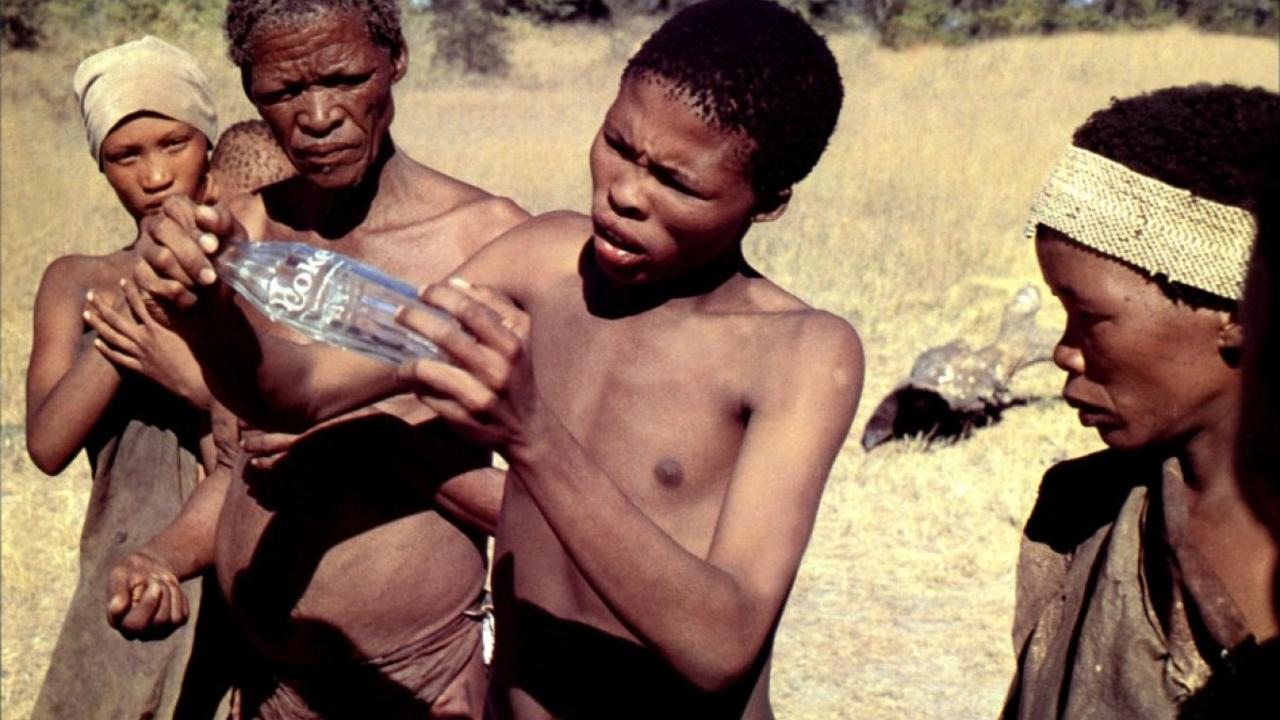
\includegraphics[width=10cm]{lahev_bohove.jpg}	\\
				Bohové musí být šílení (1980)
			\end{center}
		
		\end{frame}
	
		\begin{frame}{K přemýšlení}
			\begin{itemize}
			\item Když lidé nebudou o vašem projektu vědět, nebudou ho používat.
			\item Když lidé nebudou umět nainstalovat váš program, nebudou ho používat.
			\item Když lidé nepoznají, jak použít váš kód, nepoužijí ho.
			\item Když váš program nebude mít očekávané výsledky, lidé ho nebudou používat.
			\end{itemize}
		\end{frame}
	
    
    \section{Druhy dokumentace}
    
    	\begin{frame}{Jaký máme výběr?}
    	Mezi dokumentaci můžeme zahrnout několik různých forem:
    	\begin{itemize}
    		\item konceptuální 
    		\item procedurální 
    		\item referenční
    		\item výukovou
    	\end{itemize}
		\end{frame}
	
		\begin{frame}{Konceptuální dokumentace}
		\textbf{Konceptuální} dokumentace se snaží vysvětlit uživatelům danou problematiku (\textbf{koncept}) tak, aby tito pochopili princip fungování a potřebné souvislosti. Například:
		
		\begin{itemize}
			\item Co je počítačová síť a jak se po ní posílají datagramy?
			\item Co jsou optické vlastnosti objektivu a jak ovlivňují výsledné foto?
			\item Jak funguje útok \textit{hrubou silou} a proč je důležité volit si komplikovaná přístupová hesla?
			\item Jak působí bakterie zubního plaku a jak zvolit správný kartáček?
		\end{itemize}
		\end{frame}
	
		\begin{frame}{Procedurální dokumentace}
		\textbf{Procedurální} dokumentace poskytuje jasný návod, většinou rozdělený na jednotlivé kroky (\textbf{procedura}), ke splnění uživatelského záměru (\textbf{user case}). Mimo jiné:
	
		\begin{itemize}
			\item Jak nainstalovat aplikaci XY.
			\item Jak napsat a odeslat email pro úplné začátečníky.
			\item Jak vytvořit nového uživatele a přidělit mu patřičná systémová práva.
			\item Jak provést předletovou kontrolu osobního letadla Boeing~747.
		\end{itemize}
		\end{frame}

		\begin{frame}{Referenční dokumentace}
		\textbf{Referenční} dokumentace nabízí ucelený přehled (\textbf{referenci}) vlastností, voleb, nastavení a způsobů použití, aby si uživatel mohl sám objevit vlastní přístup a sestavit si své vlastní postupy:

		\begin{itemize}
			\item manuálové stránky v Linuxu
			\item přehled typů žárovek pro osvětlení vozidla
			\item přehled ingrediencí potřebných pro upečení dortu
			\item přehled voleb příkazu \texttt{dnf} ve Fedoře.
		\end{itemize}
		\end{frame}

  	\begin{frame}{Výuková dokumentace}
		\textbf{Výuková} dokumentace, tzv. \textbf{tutoriály}, je spojení konceptuální a procedurální stránky dokumentace, takže výsledkem není jenom splněný uživatelský záměr, ale také částečné pochopení problematiky a kontextu.
		
		\vspace{5pt}
		
		Je velmi důležité, abychom z konceptuálního hlediska vysvětlili pouze tolik, kolik je nezbytně nutné. Chceme-li pomocí tutoriálů vysvětlit širší problematiku, pak volíme několik na sebe navazujících.	
	\end{frame}

	\begin{frame}{Úkol pro vás}
	Navrhněte dokumentaci pro nějakou věc denní spotřeby. Kterou formu zvolíte? Proč?
	\end{frame}

	\section{Jak psát?}

	\begin{frame}{Správný styl dokumentace}
	V dokumentaci bychom měli zachovávat několik stylistických pravidel:
	\begin{itemize}
		\item jednoznačné výrazy
		\item jednoduché a krátké formulace
		\item neutrální výrazy
		\item genderově neutrální prvky
		\item v případě pochybností je lepší více informací než méně
		\item rozkazovací způsob (procedury)
	\end{itemize}
	\end{frame}

	\begin{frame}{Nesprávný styl dokumentace}
	V dokumentaci bychom se raději měli vyhnout:
	\begin{itemize}
		\item estetickým formám jazyka (metafory, přirovnání, nadsázka)
		\item ironii a sarkasmu
		\item humoru
		\item zlehčování problémů
		\item utěšování uživatelů
	\end{itemize}
	\end{frame}

	\begin{frame}{Porušování pravidel}
	Někdy můžeme uznat za vhodné pravidla porušit a získáme tak jinou formu dokumentace, jež je
	\begin{itemize}
		\item zajímavá
		\item neotřelá
		\item vtipná
		\item parodická
	\end{itemize}
	Je však nutné si uvědomit, kdo budou čtenáři naší dokumentace a jsou-li tito ochotni takový přístup snášet.
	\end{frame}

	\begin{frame}{Úkol pro vás}
			Jakou věc by bylo možné dokumentovat s porušením předchozích pravidel? Jakou věc byste nikdy nechtěli takto dokumentovat?
	\end{frame}

	\section{V čem psát?}

	\begin{frame}{Technické zpracování}
	Dokumentaci můžeme psát ve spoustě různých formátů. Záleží, co přesně od dokumentace očekáváme. Můžeme si vybrat na základě následujících kritérií:
	\begin{itemize}
		\item obtížnosti tvorby dokumentace (WYSIWYG, markdown, markup, \ldots{})
		\item metod zobrazení (web, čtečka, tištěné médium, audiovizuální metody)
		\item možností spolupráce (žádná, cvs, git, Google)
		\item možností publikace (ručně, automaticky (CI))
		\item dostupnosti metadat textu (sémantický markup)
	\end{itemize}
	V podstatě platí, že čím více muziky čekáme, tím více do dokumentace budeme muset investovat.
	\end{frame}

	\begin{frame}{Formáty}
	Pokud se v souvislosti s dokumentací mluví o formátech, pak máme na mysli v podstatě dva typy a to:
		\begin{itemize}
			\item \textbf{zdrojové} formáty, tedy ty, ze kterých se dokumentace překládá
			\item \textbf{cílové} formáty, tedy ty, do kterých se překládá
		\end{itemize}
	Některé souborové formáty mohou být jak zdrojové, tak cílové (HTML)
	\end{frame}

	\begin{frame}{Stručný přehled zdrojových formátů}
		\begin{itemize}
			\item čistý text
			\item markdown (Markdown, AsciiDoc)
			\item markup (HTML, XML, DocBook, Mallard, reST, \LaTeX)
			\item nativní formáty WYSIWYG aplikací (doc, docx, fm, odt, indd)
		\end{itemize}
	\end{frame}

	\begin{frame}{Stručný přehled cílových formátů}
		\begin{itemize}
			\item HTML (web)
			\item epub, mobi a další (ebooky)
			\item pdf (tiskárna)
		\end{itemize}
	\end{frame}

	\begin{frame}{Nejčastěji používané formáty}
		\begin{itemize}
			\item Markdown (Github)
			\item AsciiDoc (Red Hat)
			\item reST (Python)
			\item Mallard (Gnome)
			\item \TeX, \LaTeX
			\item DocBook (SuSE, Red Hat, IBM)
		\end{itemize}
	\end{frame}

	\begin{frame}{Markdown}
	\textbf{Výhody:}
	\begin{itemize}
		\item jednoduchý
		\item čitelný
	\end{itemize}	
	\textbf{Nevýhody:}
	\begin{itemize}
		\item omezené typografické možnosti
		\item minimální sémantika
		\item nejasné hranice mezi prvky
		\item významy některých značek kolidují s reálnými znaky (*)
	\end{itemize}				
	Markdown je vhodný především pro malé projekty, například README na Githubu.
	\end{frame}

	\begin{frame}{AsciiDoc}
	\textbf{Výhody:}
	\begin{itemize}
		\item jednoduchý a čitelný
		\item částečně programovatelný
		\item lze psát sémantický kód
	\end{itemize}	
	\textbf{Nevýhody:}
	\begin{itemize}
		\item nejasné hranice mezi prvky
		\item vlastní úpravy porušují standard (kompatibilita)
		\item sémantika zvyšuje složitost a omezuje čtivost
		\item kolidující značky
	\end{itemize}				
	AsciiDoc je vhodný pro malé i velké projekty, ale v základu postrádá některé funkce, které jiné formáty nabízejí.
	\end{frame}
    
	\begin{frame}{reST a Sphinx}
	\textbf{Výhody:}
	\begin{itemize}
		\item jednoduchý a čitelný
		\item programovatelný
		\item sémantický
		\item jasné hranice mezi prvky
	\end{itemize}	
	\textbf{Nevýhody:}
	\begin{itemize}
		\item nutnost přesně dodržovat strukturu kódu
	\end{itemize}				
	reST, a jeho rozšíření Sphinx, jsou velmi vhodné pro veškeré typy projektů. Jsou oblíbené především mezi programátory Pythonu, protože struktura formátu připomíná Python.
	\end{frame}

	\begin{frame}{Mallard}
	\textbf{Výhody:}
	\begin{itemize}
		\item sémantický
		\item jasné hranice mezi prvky
		\item modulární
	\end{itemize}	
	\textbf{Nevýhody:}
	\begin{itemize}
		\item méně přehledný a čtivý
		\item poměrně neznámý
		\item modulární
	\end{itemize}				
	Mallard byl původně určen pro psaní \textbf{Gnome} help. Je navržen pro \textit{topic based authoring} (tématicky zaměřené psaní), takže zdrojový kód se spíše skládá z fragmentovaných prvků než velkých celků.
	\end{frame}

	\begin{frame}{\TeX, \LaTeX}
	\textbf{Výhody:}
	\begin{itemize}
		\item sémantický
		\item jasné hranice mezi prvky
		\item poměrně přehledný a čtivý
		\item dlouhodobě vyvíjený
	\end{itemize}	
	\textbf{Nevýhody:}
	\begin{itemize}
		\item nehezký výstup do HTML
		\item mnoho odnoží s různými výstupy a funkcemi
	\end{itemize}				
	Sázecí systém \TeX{} a sada maker zjednodušujících práci s ním, \LaTeX, byl vyvinut pro sazbu matematických publikací. Nejlepší výsledky poskytuje pro vytváření tištěné dokumentace. 
	\end{frame}

	\begin{frame}{Docbook}
	\textbf{Výhody:}
	\begin{itemize}
		\item sémantický
		\item jasné hranice mezi prvky
		\item dlouhodobě vyvíjený, tedy robustní
		\item systém validace nedovolí chyby
	\end{itemize}	
	\textbf{Nevýhody:}
	\begin{itemize}
		\item nepřehledný
		\item mnoho různých prvků a vztahů mezi nimi
		\item vyžaduje čas na naučení
		\item neodpouští chyby
	\end{itemize}				
	Docbook je pravděpodobně nejlepší volbou pro psaní korporátní dokumentace.
	\end{frame}

	\begin{frame}{Výběr vhodného formátu}
	Před výběrem formátu pořádně zamyslet, co od něj přesně chceme, neboť špatný výběr formátu může celou tvorbu dokumentace zkomplikovat.

	Ptejme se na:
	
	\begin{itemize}
		\item formu spolupráce
		\item obtížnost psaní
		\item automatizované testování a publikování
		\item formy výstupu
		\item přenositelnost do jiných formátů
		\item budoucnost projektu
	\end{itemize}
	Obecně platí, že \textbf{čím složitější} formát, tím \textbf{více možností použití}.
	\end{frame}

	  \begin{frame}{Úkol pro vás}
			Jaký formát byste vyzkoušeli jako první, kdybyste si měli vybrat na základě poskytnutých informací? Proč?
	  \end{frame}


	\section{Praxe}	

	\begin{frame}{Obvyklý postup při vytváření dokumentace}
	Dokumentace obvykle vzniká následujícím postupem:
			\begin{enumerate}
				\item zjišťování potřeb uživatelů
				\item plánování a alokace zdrojů
				\item stanovení formy spolupráce a formátu
				\item tvorba zdrojových dokumentů
				\item překlad do cílových dokumentů
				\item publikování
				\item vyhledání a opravení chyb
				\item znovu přeložení a publikování (nová subverze)
			\end{enumerate}
	\end{frame}

\begin{frame}{Dokumentace v Red Hatu obsahově}
Red Hat v současné době udržuje několik dokumentačních projektů. Organizační struktura dokumentačního oddělení používá tři oddělené pozice:

\begin{itemize}
	\item obsahový stratég (content strategist)
	\item programový manažer (document program manager)
	\item dokumentátor (technical writer)
\end{itemize}

Každý z nich je zodpovědný za jinou oblast vývoje dokumentace, leč jejich funkce se mohou v Red Hatu překrývat, protože Red Hat pracuje na principu \textit{meritokracie} a platí, že nejlepší názor se počítá. 
\end{frame}


	\begin{frame}{Dokumentace v Red Hatu technicky}
		Z hlediska technického zpracování se používají dva postupy, které jsou založené buď na:
		
		\begin{itemize}
			\item Docbooku
			\item AsciiDocu
		\end{itemize}
	
		Docbook je v současné době na ústupu a projekty přecházejí na AsciiDoc.
	\end{frame}

	\begin{frame}{Pracovní postup v Docbooku}
	Při vytváření dokumentace psané v Docbooku se postupuje takto:

	\begin{itemize}
		\item klonování Git repozitáře
		\item ruční úprava dokumentů v textových editorech
		\item sledování změn v paralelní Git větvi (branch)
		\item validace a překlad na lokálním stroji (publican)
		\item peer review $\longrightarrow$ kontrola kvality
		\item automatizované testy obsahu (překlepy, názvy)
		\item merge do hlavní větve
		\item překlad hlavní větve (publican) a vystavení na portálu (www.redhat.com)
	\end{itemize}
	\end{frame}

	\begin{frame}{Pracovní postup v AsciiDocu}
	Při vytváření dokumentace psané v AsciiDocu se postupuje takto:

	\begin{itemize}
		\item klonování Git repozitáře
		\item ruční úprava dokumentů v textových editorech
		\item sledování změn v paralelní Git větvi (branch)
		\item validace a překlad na lokálním stroji (asciidoctor, ccutil)
		\item peer review $\longrightarrow$ kontrola kvality
		\item merge do hlavní větve
		\item překlad hlavní větve (ccutil $\longrightarrow$ publican) a vystavení na portále
	\end{itemize}
	\end{frame}

	\begin{frame}{Probíhající diskuse o dokumentaci}
	V dokumentačním týmu v současné době probíhá několik diskusí a iniciativ o tom, jak dělat věci lépe, aby zákazník dostal za svoje peníze co nejlepší službu. 
	
	\begin{itemize}
		\item spolupráce upstream $\longleftrightarrow$ downstream
		\item konzistentní terminologie (IBM Style Guide)
		\item Docbook versus AsciiDoc
		\item správný postup u peer review
		\item jednotný způsob zápisu značek u AsciiDocu
		\item sémantický zápis značek v AsciiDocu
		\item modulární dokumentace
	\end{itemize}
	\end{frame}

	\begin{frame}{Otázky}
		Kdo se moc ptá, moc se doví.
		
		\vspace{10pt}
		
		Takže?
	\end{frame}

	\begin{frame}
	Děkuji za pozornost.
	\end{frame}

\end{document}